% What we have done (data preprocessing, getting the rhythmic instrument, retrieving the tokens, baseline using dadagp (GuitarCTRL))
\subsection{DadaGP token preprocessing}
% --> Retrieving, cleaning, mapping DadaGP
% Rhythmic guitar detection (cite paper)

The DadaGP dataset provides token files containing information for all instruments in a score.
As we want to explore various conditioning combinations for tablature generation, we developed a function to extract tokens specific to selected instruments.
We considered several possible ways to perform this extraction: runnning DadaGP's token processing script for each instrument, or filtering the tokens from the complete token text file based on the instrument name.
Opening, parsing and looping on the GuitarPro file using pygp is needed for the DadaGP token processing script and is very time-consuming, much more than processing txt files.
We recall that DadaGP comprises 26,181 GuitarPro files.
Using our algorithm it only took 5min30 to process all the files and generate a copy of DadaGP containing token files of bass guitar only.
To perform this operation, we leverage the fact that tokens of a given instrument start with the instrument name followed by a colon, e.g., \texttt{bass:} for the bass guitar.
However we must be careful not to miss the potential note effect tokens that are not instrument-specific, but come right after the token they are related to.
After extracting those tokens and the general tokens (metadata tokens and wait tokens),
we sum the potential consecutive wait tokens that were previously separated by notes from instruments that are no longer present.

\begin{figure}[!ht]
    \centering
    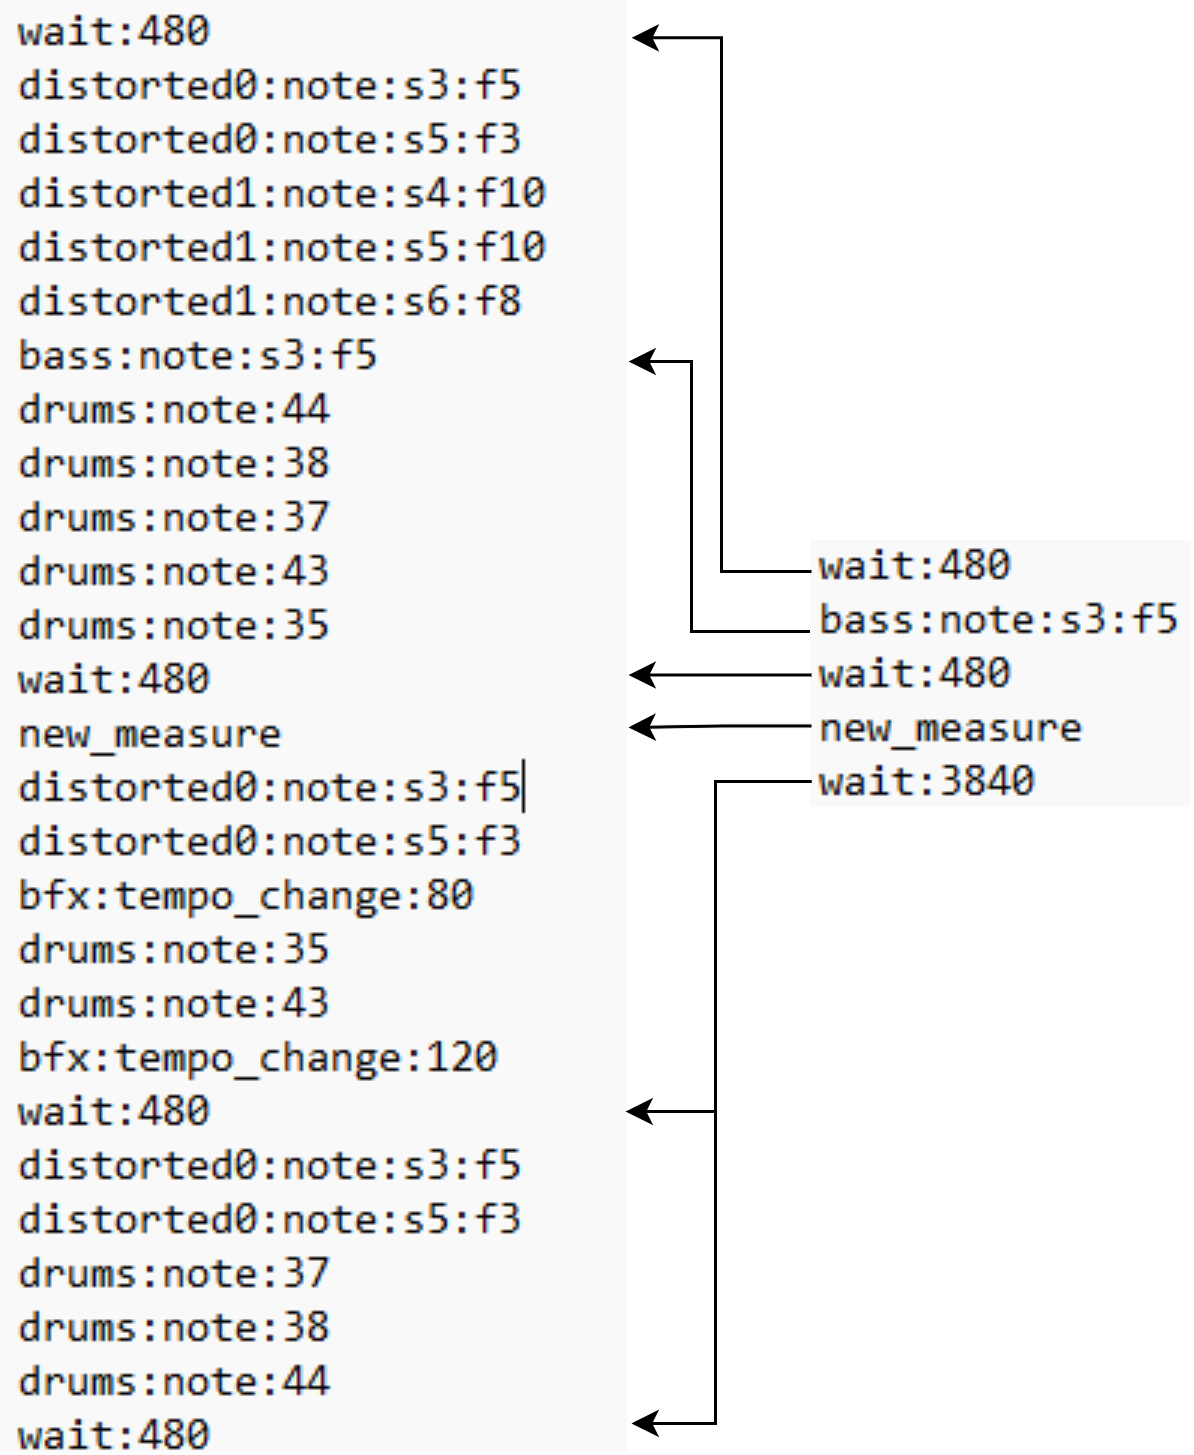
\includegraphics[width=.5\linewidth]{../images-figures/token_extraction.png}
    \caption{Example of an extraction of bass guitar token in The Strokes - Last Nite}
    \label{fig:token_extraction}
\end{figure}

An example of token extraction is shown in Figure~\ref{fig:token_extraction}.
This figure also shows the concatenation of wait tokens.
At the end of the song, the bass guitar stops playing before the other instruments.
We can notice the several \texttt{wait:480} tokens that are summed up to a single \texttt{wait:3840} token.

\subsection{Rhythmic guitar identification}

The algorithm we just presented allows us to extract tokens for any instrument in the DadaGP dataset.
In typical rock band instrumentation, rhythmic guitars complement bass guitars with their repetitive chord patterns, providing harmonic and rhythmic structure at a higher pitch \cite{regnier_identification_2021}.
This characteristic makes them particularly relevant for conditioning bass generation tasks, therefore, our first focus is on conditioning bass guitar tablature generation using the rhythmic guitar.


To identify rhythmic guitar parts in the DadaGP dataset, we implemented the method proposed by Régnier et al. \cite{regnier_identification_2021},
which uses features describing notes and chords at the bar level, along with corresponding tablatures.
Their model outputs a prediction between 0 and 1 for each bar. The closest to 1, the more likely the part is a lead on the bar, and the closest to 0, the more likely it is a rhythmic guitar part on the bar.
In their paper, they consider that a score below 0.5 correspond to a rhythmic guitar parts. We wanted to select and condition the generation on only one rhythmic guitar part, the "most" rhythmic.
Therefore, we applied the 0.5 threshold to the predictions and selected the part with the highest proportion of rhythmic bar over the course of the song.
Implementing this method required adapting their code to the DadaGP dataset.
Significant effort was spent mapping the identified rhythmic guitar parts to their respective names in the DadaGP files, as the dataset renames instruments, whereas the identification tool relies on GuitarPro part names.
Thanks to this work, we were able to extract two more datasets: one containing the rhythm guitar tokens and the other containing both the bass and the rhythmic guitar tokens.

% FIGURE EXAMPLE OF SELECTION OF RHYTHMIC GUITAR ON A SONG
\begin{figure}[!ht]
    \centering
    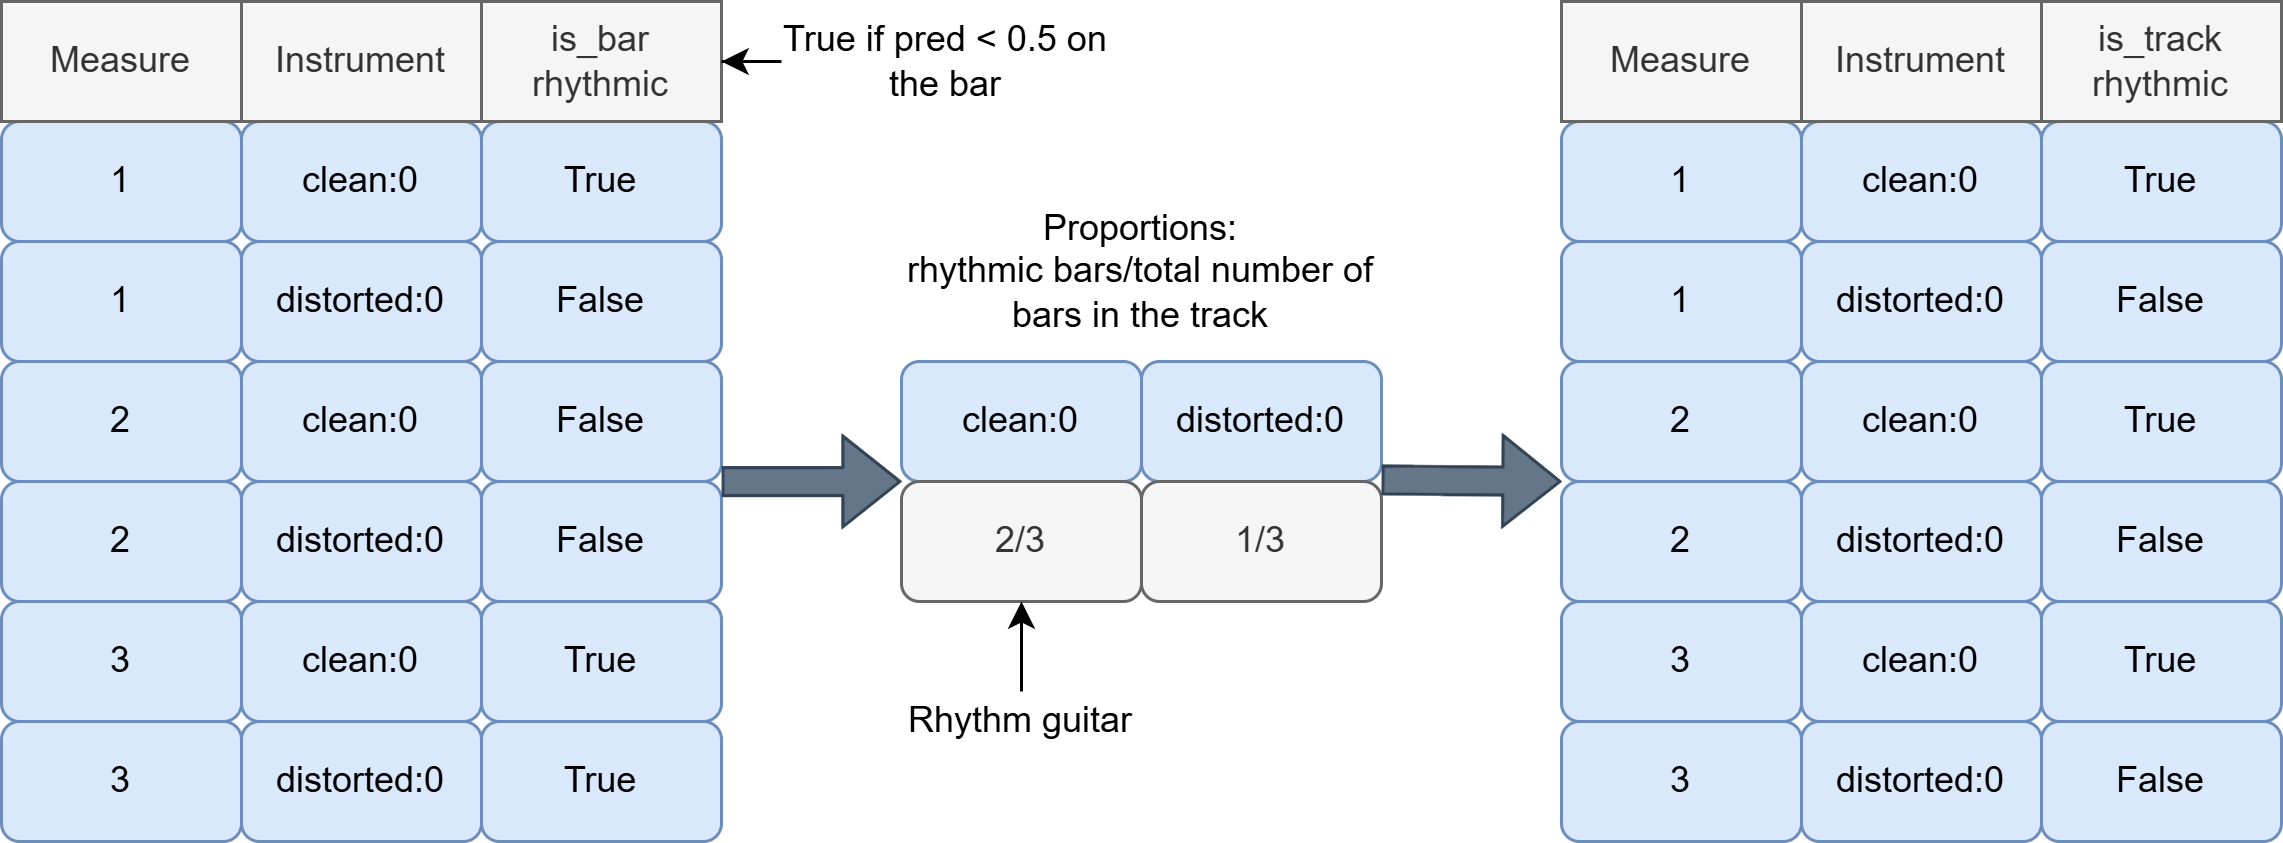
\includegraphics[width=\linewidth]{../images-figures/rhythm_guitar_selection.png}
    \caption{Example of rhythmic guitar selection after applying the method of Régnier et al.}
    \label{fig:rhythm_guitar_selection}
\end{figure}

Figure~\ref{fig:rhythm_guitar_selection} shows an example of the selection of the rhythmic guitar part.
After retrieving the instrument with the highest number of rhythmic bars over the song,
we generate a column \texttt{is\_track\_rhythmic} that is filled with 1 (or True) for the rhythmic guitar and 0 for the other instruments.


\subsection{Post processing}

To avoid too long sequences, we chose to extract samples of 16 measures from the songs.
We extract sequences with a stride of 8 measures, which allows us to have a good overlap between the sequences.
This will help the model to learn the transitions, and understand the various possible contexts around a given sequence.
Sequences also have at most 800 tokens and at least 50 tokens.
Thresholds were set to avoid training on sequences that are either too long or that does not contain rythmic guitar or bass.
These thresholds are not applied on the complete sequences containing both the tokens of the rhythmic guitar and the bass.

% FIGURE DISTRIBUTION OF SEQUENCE LENGTHS
\begin{figure}[!ht]
    \centering
    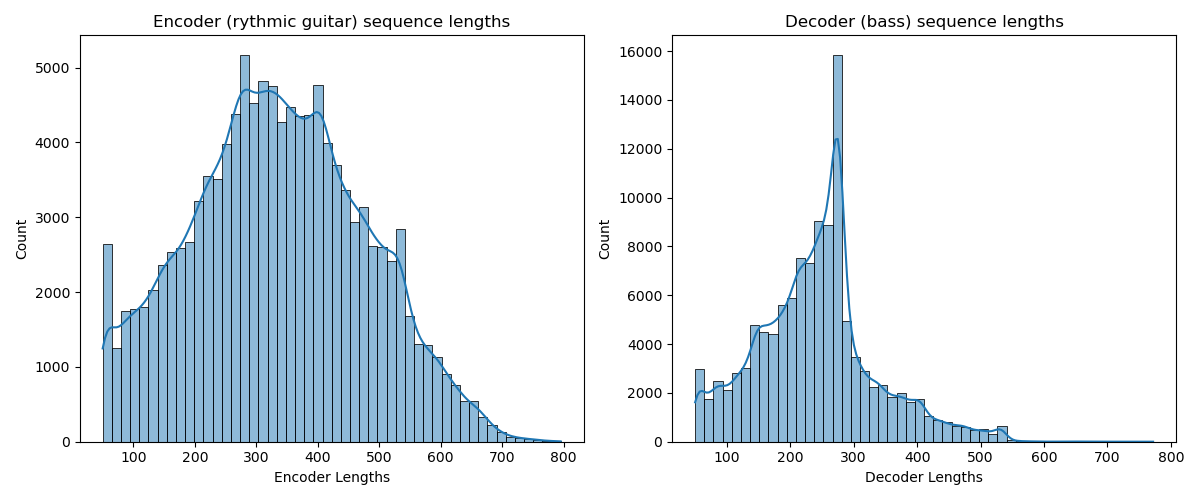
\includegraphics[width=.8\linewidth]{../images-figures/sequence_lengths_16_8_800_50.png}
    \caption{Distribution of sequence lengths in the training dataset}
    \label{fig:sequence_length_distribution}
\end{figure}

Figure \ref{fig:sequence_length_distribution} shows the distribution of sequence lengths in the training dataset.
The majority of the sequences are between 200 and 400 tokens long for the rythmic guitar and between 100 and 300 tokens long for the bass.

Those sequences fill in a dictionary with keys \texttt{Encoder\_RG}, \texttt{Decoder\_Bass} and \texttt{All\_Events}.
For instance \texttt{dict['Encoder\_RG'][i]} contains the tokens of the rhythmic guitar for the i-th sequence.
\texttt{dict['All\_Events'][i]} contains the tokens of bass guitar and rhythmic guitar for the i-th sequence.


\begin{figure}[!ht]
    \centering
    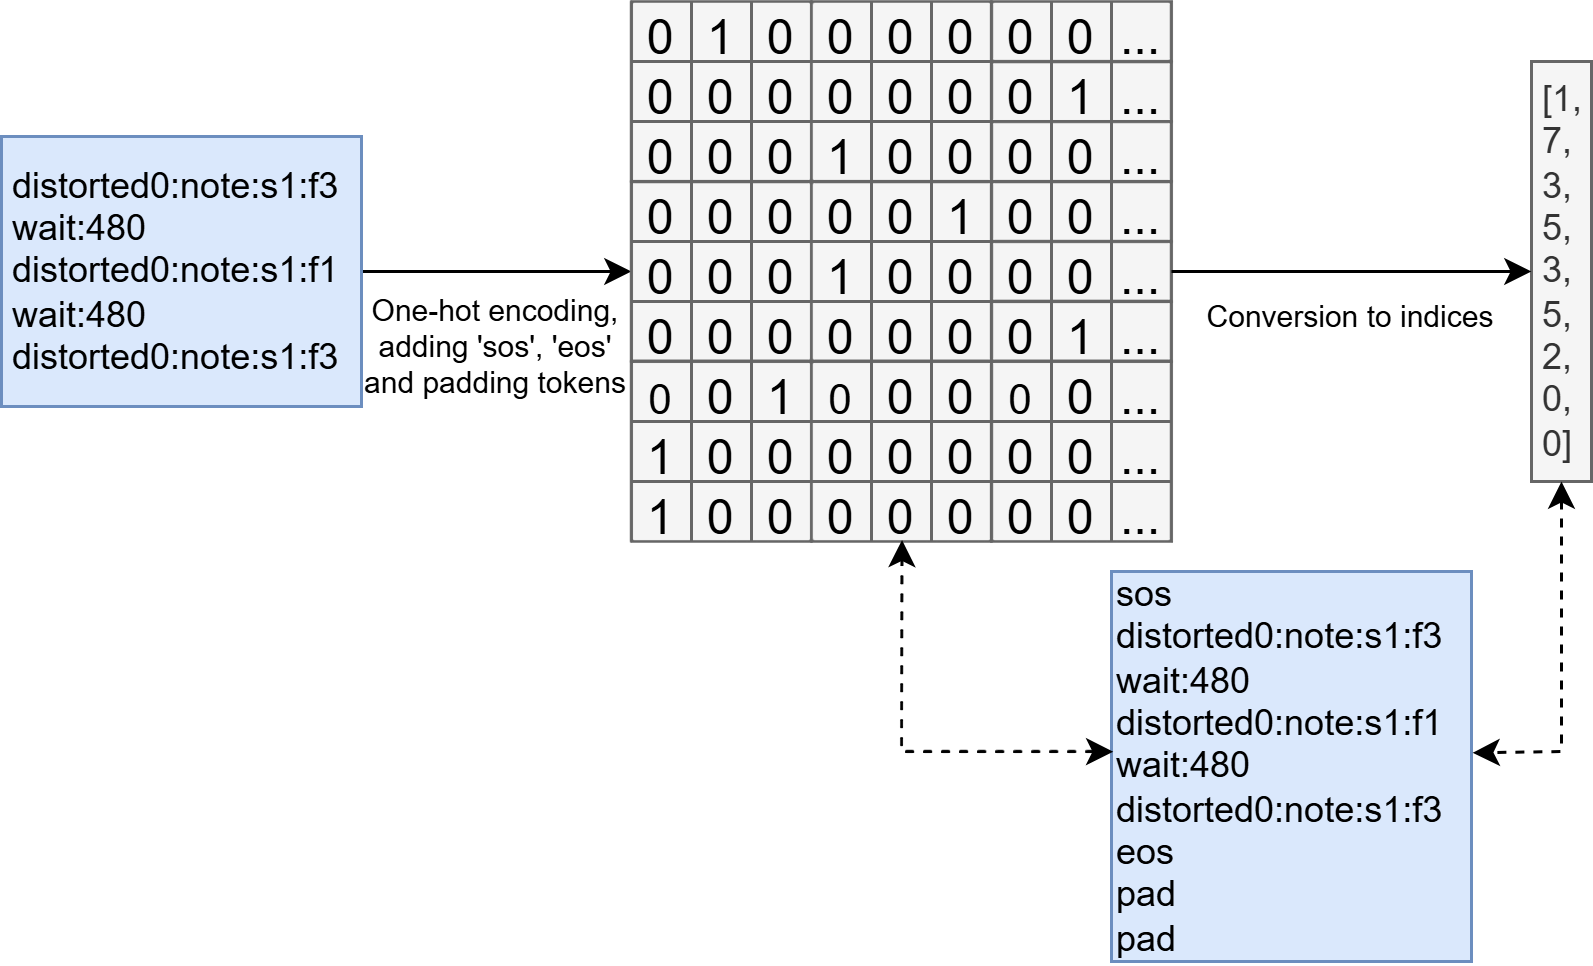
\includegraphics[width=.8\linewidth]{../images-figures/conversion_indices.png}
    \caption{Conversion from a txt token sequence to indices}
    \label{fig:conversion_indices}
\end{figure}

The sequences are then processed as described in figure \ref{fig:conversion_indices}.
They go through a one-hot encoding process, then we add 'start of sequence' and 'end of sequence',
and padding tokens after the 'eos' token to reach a fixed length of approximately 800 tokens.
The final dictionary of sequences as indices is finally split into training, validation and test sets with proportions 0.8, 0.1 and 0.1 respectively.
We generated 118 167 sequences in total, which leads to 94 533 sequences in the training set and 11 817 in both the validation and test sets.

